\chapter{Desenvolvimento do Trabalho}
\label{chap:desenvolvimento-trabalho}

Este capítulo trata da forma como o trabalho foi desenvolvido de forma a aplicar a metodologia proposta, descrevendo os processos utilizados para a verificação do desacoplamento e instabilidade do sistema (Seção \ref{sec:verificacao-desacoplamento}); a modelagem dos controladores \textit{fuzzy} (Seção \ref{sec:controlador-fuzzy}) e neuro-\textit{fuzzy} (Seção \ref{sec:controlador-neuro-fuzzy}); e a descrição detalhada dos experimentos realizados (Seção \ref{sec:experimentos-realizados}).

\section{Verificação do Desacoplamento das Entradas}
\label{sec:verificacao-desacoplamento}

\input{./02-elementos-textuais/desenvolvimento-verificacao-desacoplamento}

\section{Controladores Fuzzy}
\label{sec:controlador-fuzzy}

O projeto dos controlador \textit{fuzzy} foi focado na estabilização de atitude e altitude de um \textit{drone} sujeito a parâmetros específicos\footnote{Estes valores foram também utilizados por \citeonline{Balas2007} para definir uma especificação do sistema}, sendo eles: a gravidade $g=9,81$ m/s\textsuperscript{2}, a massa do quadricóptero $m=2,3$ kg e o comprimento de cada haste do \textit{drone} $l=0,5$ m. Um dos controladores projetado tem, como objetivo, controlar a altitude do quadricóptero, ao passo que um segundo visa a sua estabilização de sua atitude.

O controlador de altitude possui duas entradas e uma saída. As entradas são referentes à posição vertical do quadricóptero ($z$) e sua respectiva velocidade ($\dot{z}$), ao passo que a saída diz respeito ao sinal de controle a ser aplicado sobre o sistema para estabilizar sua altitude ($u_1$). Sua aplicação no sistema é mostrada na Figura \ref{fig:u1_mamdani_blocks}.

% Mostrar diagrama do sistema controlado (para ruídos), sobre a entrada u1
\begin{figure}[!htb]
    \centering
    \caption{Diagrama do sistema de controle de altitude utilizando controlador fuzzy}
    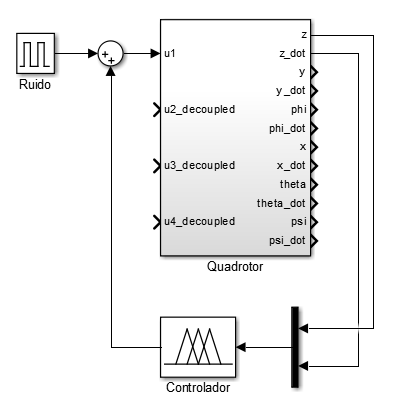
\includegraphics[width=0.5\textwidth]{./04-figuras/resultados/novos/simulink_printscreen_z}
    \label{fig:u1_mamdani_blocks}
\end{figure}

Utilizando o \textit{Fuzzy Logic Toolbox} do MATLAB, cada variável linguística do controlador fuzzy foi divida em três conjuntos: N (negativo), Z (zero) e P (positivo), tomando como base os trabalhos de \citeonline{Maj2013} e \citeonline{Gao2014Stability}. As regras fuzzy definidas para este controlador são mostradas no Quadro \ref{qua:regras_fuzzy_u1_mamdani}, e a Figura \ref{fig:1_mamdani_surface} exibe seu equivalente em superfície.

% Mostrar regras Fuzzy envolvidas no controle de u1 (quadro de regras + superfície)
% Tá errada!
\begin{quadro}[!htb]
    \centering
    \caption{Regras fuzzy para modelagem do controle de altitude\label{qua:regras_fuzzy_u1_mamdani}}
    \begin{tabular}{|c|c|c|}
    % \begin{tabular}{>{\centering\bfseries}m{1in} >{\centering}m{1in}
        \hline
        \textbf{{$z$}} & 
        \textbf{{$\dot{z}$}} &
        \textbf{{$u_1$}} \\
        \hline %01
            N &
            - &
            N \\
        \hline %02
            P &
            - &
            P \\
        \hline %03
            Z &
            N &
            N \\
        \hline %04
            Z &
            Z &
            Z \\
        \hline %05
            Z &
            P &
            P \\
        \hline
    \end{tabular}
    % \begin{TAB}(r,1cm,2cm)[5pt]{|c|c|}{|c|c|c|}% (rows,min,max)[tabcolsep]{columns}{rows}
    %     hi & tall one    \\
    %     hi & medium one  \\
    %     hi & standard one\\
    % \end{TAB}
\end{quadro}


\begin{figure}[!htb]
    \centering
    \caption{Superfície das regras do sistema de controle fuzzy para a altitude do quadrotor}
    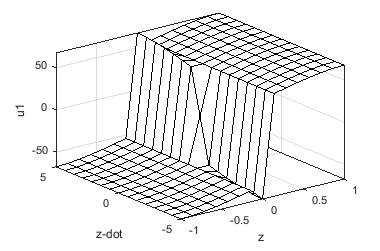
\includegraphics[width=0.6\textwidth]{./04-figuras/resultados/fis_u1/u1_mamdani_surface}
    \label{fig:1_mamdani_surface}
\end{figure}

O controlador de atitude projetado também possui duas entradas e uma saída. Desta vez, entretanto, as entradas são referentes ao ângulo em relação ao eixo horizontal ($\phi$ ou $\theta$) e sua respectiva variação ($\dot{\phi}$ ou $\dot{\theta}$). Mais uma vez, cada variável linguística foi dividida em três conjuntos: N, Z e P.

As regras que regem o controlador de atitude são sintetizadas no Quadro \ref{qua:regras_fuzzy_u2_u3_mamdani} e podem ser vistas na superfície de regras mostradas na Figura \ref{fig:u2_u3_mamdani_surface}.

% Mostrar regras Fuzzy envolvidas no controle de u2 e u3 (quadro de regras + superfície)
\begin{quadro}[!htb]
    \centering
    \caption{Regras fuzzy para modelagem do controle de atitude\label{qua:regras_fuzzy_u2_u3_mamdani}}
    \begin{tabular}{|c|c|c|}
    % \begin{tabular}{>{\centering\bfseries}m{1in} >{\centering}m{1in}
        \hline
        \textbf{{$\phi/\theta$}} & 
        \textbf{{$\dot{\phi}/\dot{\theta}$}} &
        \textbf{{$u_2/u_3$}} \\
        \hline %01
            P &
            P &
            N \\
        \hline %02
            P &
            Z &
            N \\
        \hline %03
            P &
            N &
            Z \\
        \hline %04
            N &
            N &
            P \\
        \hline %05
            N &
            Z &
            P \\
        \hline %06
            N &
            P &
            Z \\
        \hline %07
            Z &
            Z &
            Z \\
        \hline %08
            Z &
            N &
            P \\
        \hline %09
            Z &
            P &
            N \\
        \hline
    \end{tabular}
    % \begin{TAB}(r,1cm,2cm)[5pt]{|c|c|}{|c|c|c|}% (rows,min,max)[tabcolsep]{columns}{rows}
    %     hi & tall one    \\
    %     hi & medium one  \\
    %     hi & standard one\\
    % \end{TAB}
\end{quadro}


\begin{figure}[!htb]
    \centering
    \caption{Superfície das regras do sistema de controle fuzzy para a atitude do quadrotor}
    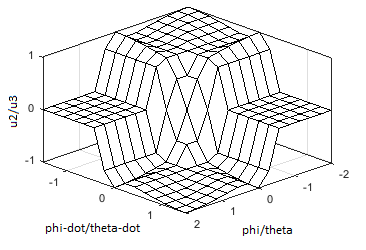
\includegraphics[width=0.6\textwidth]{./04-figuras/resultados/fis_u2/u2_u3_mamdani_surface}
    \label{fig:u2_u3_mamdani_surface}
\end{figure}

Já as Figuras \ref{fig:u2_mamdani_blocks} e \ref{fig:u3_mamdani_blocks} exibem os diagramas do sistema controlado, com atuação sobre os ângulos $\phi$ e $\theta$, respectivamente.

% Mostrar diagrama do sistema controlado (para ruídos), sobre as entradas u2 e u3
\begin{figure}[!htb]
    \centering
    \caption{Diagrama do sistema de controle de atitude utilizando controlador fuzzy sobre o ângulo $\phi$}
    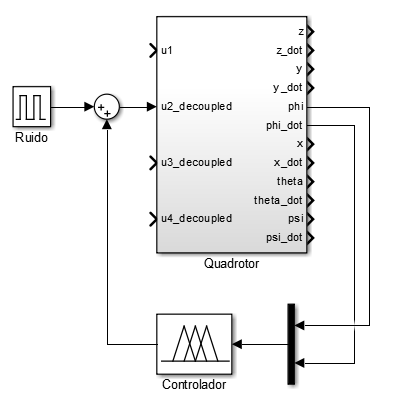
\includegraphics[width=0.6\textwidth]{./04-figuras/resultados/novos/simulink_printscreen_phi}
    \label{fig:u2_mamdani_blocks}
\end{figure}

\begin{figure}[!htb]
    \centering
    \caption{Diagrama do sistema de controle de atitude utilizando controlador fuzzy sobre o ângulo $\theta$}
    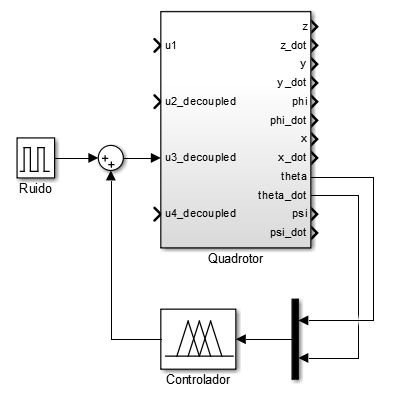
\includegraphics[width=0.5\textwidth]{./04-figuras/resultados/novos/simulink_printscreen_theta}
    \label{fig:u3_mamdani_blocks}
\end{figure}









\section{Controladores Neuro-Fuzzy}
\label{sec:controlador-neuro-fuzzy}

A partir dos controladores de atitude e altitude \textit{fuzzy} projetados, foram propostos dois controladores do tipo neuro-\textit{fuzzy}: um para cada dos casos.

Para tanto, foram utilizados os códigos mostrados nos Apêndices \ref{chap:train-anfis-altitude} e \ref{chap:train-anfis-atitude}. No processo de criação do controlador de altitude neuro-\textit{fuzzy}, foram gerados trezentos\footnote{Este valor foi arbitrado por corresponder a uma quantidade razoável para treinar a RNA sem que se alcance o sobre-parametrização, conhecido como \textit{overfitting}.} pares de entradas e cada um deles foi submetido ao processo de inferência \textit{fuzzy} utilizando o controlador previamente modelado e descrito na Seção \ref{sec:controlador-fuzzy}. Dois terços desses dados foram utilizados para gerar o conjunto de treinamento, representado pela variável {\ttfamily train} e o um terço restante foi armazenado na variável {\ttfamily test} e utilizado para validação do treinamento. Então, utilizando o comando {\ttfamily mam2sug} do MATLAB, foi gerado um modelo fuzzy Sugeno a partir do Mamdani que havia sido modelado e este novo arquivo foi salvo sob o nome {\ttfamily fis\_altitude\_neuro.fis}.

Feito isto, utilizou-se o comando comando {\ttfamily anfisedit} para abrir o \textit{Neuro-Fuzzy Designer} do MATLAB, cuja interface é mostrada na Figura \ref{fig:anfisedit_screen}. No campo marcado pelo número 2 na imagem (\textit{Generate FIS}), clicou-se no botão \textit{Load} e se selecionou o arquivo {\ttfamily fis\_altitude\_neuro.fis} que fora gerado pelo código executado. Após isto, no campo marcado pelo número 1 (\textit{Load Data}), marcou-se \textit{Training} e \textit{worksp} para utilizar uma variável da área de trabalho do MATLAB para treinar a rede. Após clicar em \textit{Load Data}, digitou-se {\ttfamily train}, nome da variável definida no código. Então, no campo marcado pelo número 3, marcou-se \textit{Training Data} e se clicou no botão \textit{Test Now} para executar o treinamento da rede. Após estes passos, a rede neuro-fuzzy foi devidamente treinada e sua estrutura, mostrada na Figura \ref{fig:rna_anfis_altitude_gray}, pode ser obtida clicando no botão \textit{Structure} logo acima do campo 3. Esta estrutura relaciona as variáveis de entrada e suas funções de pertinência, através das regras fuzzy, à saída do sistema e às suas funções de pertinência, em que cada componente representa um neurônio da RNA obtida. 

\begin{figure}[!htb]
    \centering
    \caption{Interface gráfica da ferramenta \textit{Neuro-Fuzzy Designer} com destaque aos três campos necessários para treinamento e teste da rede neuro-fuzzy}
    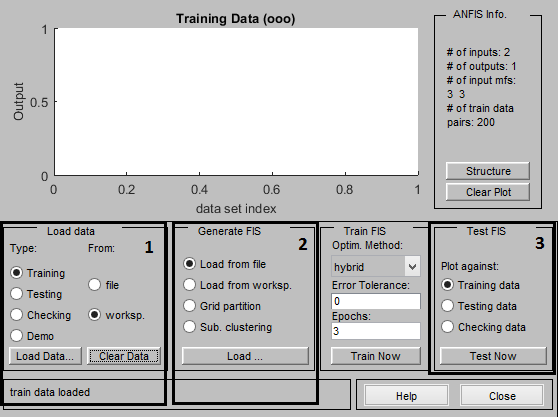
\includegraphics[width=0.8\textwidth]{./04-figuras/anfisedit/anfisedit_screen}
    \label{fig:anfisedit_screen}
\end{figure}

\begin{figure}[!htb]
    \centering
    \caption{Diagrama da RNA referente ao controlador neuro-fuzzy para altitude}
    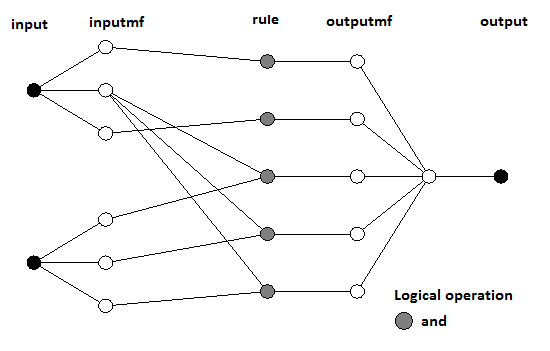
\includegraphics[width=0.6\textwidth]{./04-figuras/anfisedit/rna_anfis_altitude_gray}
    \label{fig:rna_anfis_altitude_gray}
\end{figure}

Após o término do treinamento, deve-se submeter a rede ao processo de teste. Para tanto, basta selecionar \textit{Testing} no campo marcado pelo número 1, deixar marcada a opção \textit{workspace}, clicar no botão \textit{Load Data} e escolher a variável {\ttfamily test}, que também foi definida no código executado.

A Figura \ref{fig:rna_anfis_train_result_altitude} mostra o gráfico obtido na ferramenta após o processo de treinamento, em que os círculos brancos mostram os dados utilizados no treinamento e os asteriscos pretos indicam o valor referentes a eles obtidos pela rede treinada.

\begin{figure}[!htb]
    \centering
    \caption{Resultado obtido pelo treinamento da RNA para controle de altitude}
    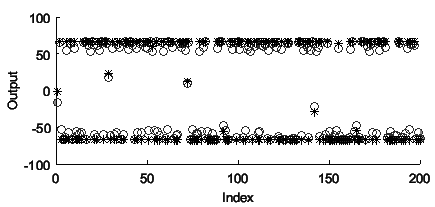
\includegraphics[width=0.6\textwidth]{./04-figuras/anfisedit/rna_anfis_train_result_altitude}
    \label{fig:rna_anfis_train_result_altitude}
\end{figure}

%Feito isto, após utilizar o comando {\ttfamily anfisedit} para abrir o \textit{Neuro-Fuzzy Designer} do MATLAB, carregou-se, nesta ferramenta, o arquivo {\ttfamily fis\_altitude\_neuro.fis} como sistema a ser treinado e, utilizando as variáveis {\ttfamily train} e {\ttfamily test}, o sistema foi devidamente treinado e validado. Após este processo, obteve-se um controlador neuro-fuzzy cujo funcionamento é mostrado pela superfície de regras mostradas na Figura \ref{fig:u1_sugeno_surface}.

Um processo similar foi aplicado para modelar o controlador de atitude neuro-fuzzy, como mostra o Apêndice \ref{chap:train-anfis-atitude}. As Figuras \ref{fig:rna_anfis_atitude_gray} e \ref{fig:rna_anfis_train_result_atitude} mostram o diagrama da RNA referente ao controlador neuro-fuzzy para atitude e o resultado obtido pelo seu treinamento respectivamente.

\begin{figure}[!htb]
    \centering
    \caption{Diagrama da RNA referente ao controlador neuro-fuzzy para atitude}
    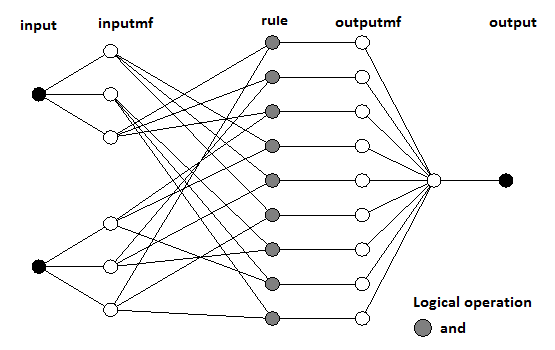
\includegraphics[width=0.6\textwidth]{./04-figuras/anfisedit/rna_anfis_atitude_gray}
    \label{fig:rna_anfis_atitude_gray}
\end{figure}

\begin{figure}[!htb]
    \centering
    \caption{Resultado obtido pelo treinamento da RNA para controle de atitude}
    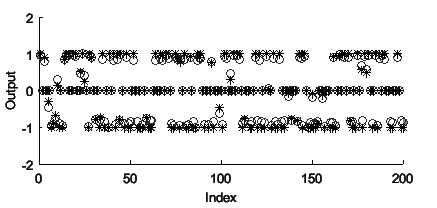
\includegraphics[width=0.6\textwidth]{./04-figuras/anfisedit/rna_anfis_train_result_atitude}
    \label{fig:rna_anfis_train_result_atitude}
\end{figure}

O processo de treinamento determina o comportamento dos controladores neuro-fuzzy projetados, cujas superfícies de regras são exibidas nas Figuras \ref{fig:u1_sugeno_surface} e \ref{fig:u2_u3_sugeno_surface}.

%-----
%Utilizando o comando {\ttfamily mam2sug} do MATLAB, obteve-se um novo modelo fuzzy do tipo Sugeno para cada modelo previamente definidos: um para controle de altitude e um segundo para controle de atitude do quadrotor. Então, utilizando o \textit{Neuro-Fuzzy Designer} do MATLAB, cada um dos modelos Sugeno criados foi treinado a partir de resultados obtidos pelos modelos fuzzy previamente elaborados. Não houve nenhuma alteração nas regras dos sistema, mas, devido às generalizações e aprendizagem da rede neuro-fuzzy, a relação entre valores de cada conjunto de saída foi ligeiramente alterado. Isso pode ser visto a partir das superfícies de regras para ambos os controladores, mostradas nas Figuras \ref{fig:u1_sugeno_surface} e \ref{fig:u2_u3_sugeno_surface}.

% Mostrar superfície Sugeno
\begin{figure}[!htb]
    \centering
    \caption{Superfície das regras do sistema de controle neuro-fuzzy para a altitude do quadrotor}
    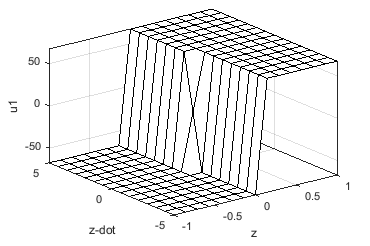
\includegraphics[width=0.6\textwidth]{./04-figuras/resultados/fis_u1/u1_sugeno_surface}
    \label{fig:u1_sugeno_surface}
\end{figure}

\begin{figure}[!htb]
    \centering
    \caption{Superfície das regras do sistema de controle fuzzy para a atitude do quadrotor}
    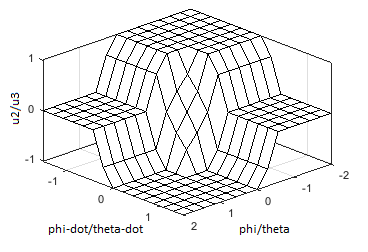
\includegraphics[width=0.6\textwidth]{./04-figuras/resultados/fis_u3/u2_u3_sugeno_surface}
    \label{fig:u2_u3_sugeno_surface}
\end{figure}




\section{Experimentos Realizados}
\label{sec:experimentos-realizados}

O primeiro experimento feito foi para mostrar a instabilidade do sistema, mostrando a resposta das variáveis relacionadas à atitude (ângulos $\phi$ e $\theta$) e altitude ($z$) quando o sistema é submetido a um breve impulso em suas entradas, simulando qualquer força que possa atuar brevemente sobre o quadrotor, como um golpe sofrido por qualquer objeto que colida com ele. Após contextualizada a necessidade de controladores, passou-se à sua implementação e uso.

Uma vez projetados os controladores fuzzy e neuro-fuzzy, o sistema foi sujeitado a distúrbios em atitude e altitude para verificar o funcionamento deles sob condições similares às mostradas quando nenhum controle agia sobre ele fazendo com que o sistema divergisse.. Primeiramente, o comportamento de ambos os controladores foi verificado quando atuando sobre o sistema para os quais eles foram projetados, com $g=9,81$ $m/s^2$, $m=2,3$ $kg$ e $l=0,5$ $m$. 

Em seguida, para testar a robustez de cada controlador, foi feita uma simulação em que eles atuam sobre um sistema cuja massa do quadrotor é $m=5$ $kg$, valor este que foi escolhido por variar o parâmetro massa em mais de 100 \%.

Os resultados obtidos são mostrados no capítulo seguinte.


%
%O desenvolvimento do trabalho se deu integralmente em ambiente simulado. Para a implementação das simulações, foi utilizado o software MATLAB\textregistered, devido à grande gama de possibilidades que ele oferece para lidar com sistemas não lineares além do excelente material de apoio da própria MathWorks\textregistered\ e da comunidade de usuários. As ferramentas do MATLAB utilizadas foram:
%\begin{itemize}
%  \item Simulink: utilizado para modelar sistemas em diagramas de blocos e fazer simulações dos sistemas resultantes;
%  \item Fuzzy Logic Toolbox: utilizado para desenvolver controladores Fuzzy.
%  \item Neuro-Fuzzy Designer: utilizado para treinar e validar controladores Neuro-Fuzzy.
%\end{itemize}
%
%\section{Contextualização do Controle de Sistemas Dinâmicos Não Lineares}
%\label{sec:metodologia-contextualizacao}
%
%Para a contextualização da ação de controle sobre sistemas não lineares, escolheu-se o sistema de pêndulo invertido por ser análogo ao modelo do \textit{drone}. Esta escolha foi baseada no fato de este sistema ser considerado um problema clássico de sistema não linear instável, sendo retratado repetidamente na literatura, como em \cite[p.~68]{Ogata2010} e em \cite[p.~186]{Dorf2011}, além de ser largamente usado como \textit{benchmark} para comparação de eficiência de variados métodos de controle, sendo alvo de estudo em diversos artigos. O primeiro passo para seu estudo é a sua modelagem matemática.

\subsection{Modelagem Matemática}
\label{subsec:sistemas-pendulum-mathematical-model}

Considerando o diagrama de corpo livre mostrado na \autoref{fig:Ogata2010_inverted_pendulum_diagram_complete}-b e se utilizando de desenvolvimento matemático chegou-se às seguintes equações para descrever o movimento do sistema do pêndulo invertido sobre o carro:
\begin{equation} \label{eq:modeling_pendulum_eq1}
	(M+m)\ddot{x} + ml\ddot{\theta} = u
\end{equation}
\begin{equation} \label{eq:modeling_pendulum_eq2}
	(I+ml^2)\ddot{\theta} + ml\ddot{x} = mlg\theta
\end{equation}
 
Em que $I$ é o momento de inércia da haste.

A partir de manipulação matemática, as equações \ref{eq:modeling_pendulum_eq1} e \ref{eq:modeling_pendulum_eq2} podem ser reescritas como:
\begin{equation} \label{eq:modeling_pendulum_eq1_modified}
	Ml\ddot{\theta} = (M+m)g\theta - u
\end{equation}
\begin{equation} \label{eq:modeling_pendulum_eq2_modified}
	M\ddot{x} = u - mg\theta
\end{equation}

A partir da \autoref{eq:modeling_pendulum_eq2_modified}, \citeonline[p.~71]{Ogata2010} obtém a função de transferência da planta como:
\begin{align} \label{eq:modeling_pendulum_tf}
\frac{\Theta(s)}{-U(s)} &= \frac{1}{Mls^2-(M+m)g} \nonumber \\
						&= \frac{1}{Ml(s+\sqrt{\frac{M+m}{Ml}g})(s-\sqrt{\frac{M+m}{Ml}g})}
\end{align}

Na \autoref{eq:modeling_pendulum_tf}, verifica-se que a planta do pêndulo invertido possui um polo no eixo real negativo e outro no eixo real positivo. Estes polos são: 
\begin{equation} \label{eq:modeling_pendulum_tf_neg_pole}
	s = -\sqrt{\frac{M+m}{Ml}g}
\end{equation}
\begin{equation} \label{eq:modeling_pendulum_tf_pos_pole}
	s = \sqrt{\frac{M+m}{Ml}g}
\end{equation}

Por possuir um polo no eixo real positivo, definido pela \autoref{eq:modeling_pendulum_tf_pos_pole}, a planta é instável em malha aberta.

\subsection{Representação no Espaço de Estados}
\label{subsec:sistemas-inverted-pendulum-state-spaces}
Para a representação do sistema no espaço de estados, em \cite[p.~71]{Ogata2010} as variáveis de estado $x_1$, $x_2$, $x_3$ e $x_4$ foram definidas como:
\begin{align*}
	x_1 &= \theta \\
	x_2 &= \dot{\theta} \\
	x_3 &= x \\
	x_4 &= \dot{x}
\end{align*}

Com isto, se obtém o vetor de estados $X$ definido por:
\begin{equation*}
X=
\left[ \begin{array}{@{}*{4}{c}@{}}
     \theta & \dot{\theta} & x & \dot{x} \\
\end{array} \right]^T
\end{equation*}

Além disto, o vetor $y$ de saída do sistema foi definido como:
\[
	y = 
	\begin{bmatrix}
		y_1 \\
		y_2
	\end{bmatrix} = 
	\begin{bmatrix}
			\theta \\
			x
	\end{bmatrix} =
	\begin{bmatrix}
			x_1\\
			x_3
	\end{bmatrix}
\]

A partir de novas manipulações matemáticas, mostra-se que a representação por espaço de estados deste sistema de pêndulo invertido pode ser definido como:
\begin{align} \label{eq:space_state_equation_pendulum}
	\dot{x} &= Ax + Bu \\
	y		&= Cx + Du
\end{align}

Em que:
\[
	A = 
	\begin{bmatrix}
		0 & 1 & 0 & 0 \\
		\frac{M+m}{Ml}g & 0 & 0 & 0 \\
		0 & 0 & 0 & 1 \\
		-\frac{m}{M}g & 0 & 0 & 0
	\end{bmatrix}\quad
	B = 
	\begin{bmatrix}
		0 \\
		-\frac{1}{Ml} \\
		0 \\
		\frac{1}{Ml}
	\end{bmatrix}
\]

\[
	C = 
		\begin{bmatrix}
			1 & 0 & 0 & 0 \\
			0 & 0 & 1 & 0
		\end{bmatrix}\quad
	D = 
		\begin{bmatrix}
			0 \\
			0
		\end{bmatrix}
\]

Desta forma, se obtém a representação completa do sistema de pêndulo invertido no espaço de estados.

\subsection{Experimentos Realizados}
\label{subsec:metodolgoia-pendulum-experimentos}

Uma variação do algoritmo presente em \cite[p.~750]{Ogata2010} foi usado para simular a resposta do sistema de pêndulo invertido a uma entrada em degrau unitário em duas situações: sem nenhuma ação de controle; e com uma ação de controle tradicional. Neste segundo caso, foi utilizado um servo sistema tipo 1, como mostrado na \autoref{fig:Ogata2010_servo_system_type_1}.

\begin{figure}[!htb]
    \centering
    \caption{Diagrama de blocos representando o sistema de pêndulo invertido controlado por um servo sistema tipo 1}
    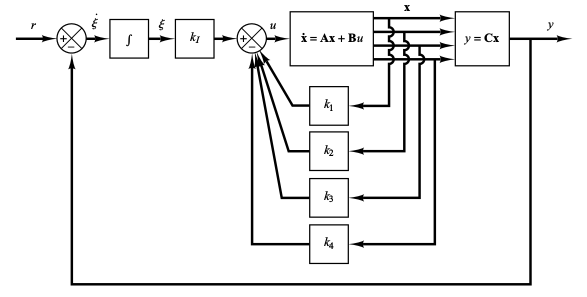
\includegraphics[width=1\textwidth]{./04-figuras/Ogata2010_servo_system_type_1}
    \fonte{\cite[p.~747]{Ogata2010}}
    \label{fig:Ogata2010_servo_system_type_1}
\end{figure}

Os parâmetros do controlador utilizados foram \cite[p.~749]{Ogata2010}:
\[
	k = 
		\begin{bmatrix}
			k_1 &
			k_2 &
			k_3 &
			k_4
		\end{bmatrix} =
		\begin{bmatrix}
			-157,6336 &
			-35,3733 &
			-56,0652 &
			50,9684
		\end{bmatrix}
\]

e
\[
k_I = -50,9684
\]

O algoritmo que implementa o sistema do pêndulo invertido e também o controlador proposto é mostrado no Apêndice \ref{chap:apendicex-pendulum-modelagem-controle}. O intuito desta etapa é mostrar a instabilidade do sistema, que diverge ao sofrer qualquer perturbação, e a ação de controle que estabiliza este sistema, tornando-o estável, fazendo com que ele não mais divirja quando perturbado.

O diagrama de blocos do sistema desenvolvido para representar o pêndulo invertido é mostrado na \autoref{fig:simulink-pendulo-diagrama-geral}. Como se pode ver, este sistema possui uma única entrada, $u$, referente à força aplicada sobre o carro, e quatro saídas: theta ($\theta$) representando o ângulo da haste do pêndulo em relação ao eixo vertical; theta\_dot ($\dot{\theta}$), a taxa de variação deste ângulo; x, a posição do carro sobre o eixo horizontal; e x\_ponto ($\dot{x}$), sua velocidade sobre este mesmo eixo.

\begin{figure}[!htb]
    \centering
    \caption{Diagrama de blocos representando o sistema de pêndulo invertido}
    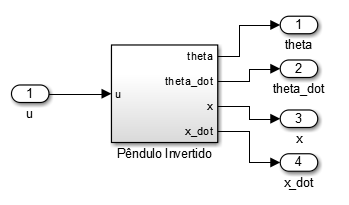
\includegraphics[width=.6\textwidth]{./04-figuras/simulink_pendulo/diagrama_geral}
    \label{fig:simulink-pendulo-diagrama-geral}
\end{figure}

A estrutura do primeiro experimento realizado é mostrado na \autoref{fig:simulink-pendulo-diagrama-geral-step}. Como se pode ver, foi aplicada à entrada $u$ do sistema, uma entrada em degrau unitário. Neste experimento, são verificadas as resposta de todas as saídas a esta excitação na entrada. Para permitir uma clara distinção da resposta do sistema sem a excitação e com ela, foi definido que ela ocorresse no tempo $t=10\ s$.

\begin{figure}[!htb]
    \centering
    \caption{Diagrama de blocos representando experimento realizado com o sistema de pêndulo invertido}
    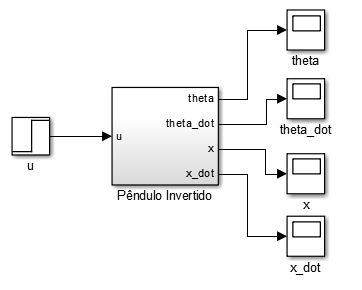
\includegraphics[width=.6\textwidth]{./04-figuras/simulink_pendulo/diagrama_step_u}
    \label{fig:simulink-pendulo-diagrama-geral-step}
\end{figure}

A estrutura do segundo experimento é análoga à do primeiro. Uma excitação em degrau é aplicada na entrada e todos os estados são verificados. Para este experimento, entretanto, a estrutura inclui um servo sistema tipo um, como mostrado na \autoref{fig:Ogata2010_servo_system_type_1},  para estabilizar o pêndulo.

%
%\section{Modelagem e Controle do Quadrotor}
%\label{sec:metodologia-quadcopter}
%
%A modelagem matemática utilizada para um quadrotor neste trabalho foi a proposta por \citeonline{Balas2007}, devido à sua abordagem completa incluindo diferentes estágios: desacoplamento das entradas, dinâmicas dos rotores e modelagem do quadrotor em si. A estrutura utilizada nesta modelagem é mostrada na \autoref{fig:Balas2007_diagram_blocos_drone_abordagem_engenharia}.

\begin{figure}[!htb]
    \centering
    \caption{Diagrama de blocos do sistema de representação de um quadricóptero}
    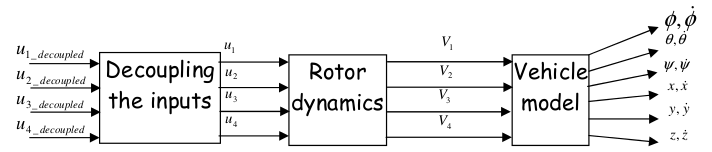
\includegraphics[width=1\textwidth]{./04-figuras/Balas2007_diagram_blocos_drone_abordagem_engenharia}
    \fonte{\citeonline[p.~58]{Balas2007}}
    \label{fig:Balas2007_diagram_blocos_drone_abordagem_engenharia}
\end{figure}

Nesta estrutura, $u_1$ representa o empuxo total sobre o quadricóptero, $u_2$ representa o momento de \textit{roll} (em torno do eixo $x$), $u_3$ representa o momento de \textit{pitch} (em torno do eixo $y$) e $u_4$ representa o momento de \textit{yaw} (em torno do eixo $z$). $u_{2\textunderscore decoupled}$, $u_{3\textunderscore decoupled}$ e $u_{4\textunderscore decoupled}$ são combinações de $u_2$, $u_3$ e $u_4$ de tal forma que as entradas $u_{2\textunderscore decoupled}$, $u_{3\textunderscore decoupled}$ e $u_{4\textunderscore decoupled}$ tenham as mesmas direções que os ângulos de Euler, $\phi$, $\theta$ e $\psi$, respectivamente. A relação entre estas entradas é dada, em \cite[p.~49]{Balas2007} por:
\[
	\begin{bmatrix}
		u'_{2} \\
		u'_{3} \\
		u'_{4}
	\end{bmatrix} = 
	\begin{bmatrix}
		cos_{\psi_{0}} & sen_{\psi_{0}}cos_{\phi_{0}}\frac{I_{xx}}{I_{yy}} & 
		0 \\
		
		-sen_{\psi_{0}}\frac{I_{yy}}{I_{xx}} &
		cos_{\psi_{0}}cos_{\phi_{0}} &
		0 \\
		
		0 &
		-sen_{\phi_{0}}\frac{I_{zz}}{I_{yy}} &
		1
	\end{bmatrix}
	\begin{bmatrix}
		u'_{2\textunderscore decoupled} \\
		u'_{3\textunderscore decoupled} \\
		u'_{4\textunderscore decoupled}
	\end{bmatrix}
\]

$I_{xx}$, $I_{yy}$ e $I_{zz}$ representam o momento de inércia do quadricóptero ao longo dos eixos $x$, $y$ e $z$, respectivamente.

Na \autoref{fig:Balas2007_diagram_blocos_drone_abordagem_engenharia}, o primeiro bloco, referente ao desacoplamento das entradas, atua justamente convertendo as entradas $u_{1\textunderscore decoupled}$ $u_{2\textunderscore decoupled}$, $u_{3\textunderscore decoupled}$ e $u_{4\textunderscore decoupled}$ de forma a se obter $u_1$, $u_2$, $u_3$ e $u_4$ para que, no bloco seguinte, de dinâmicas dos rotores, as entradas sejam, de forma isolada, o empuxo total sobre o quadricóptero e os momentos de \textit{roll}, \textit{pitch} e \textit{yaw}. Neste bloco, estabelece-se uma relação entre essas quatro entradas e a tensão que deve ser aplicada a cada um dos rotores, $V_1$, $V_2$, $V_3$ e $V_4$.

Por fim, o último bloco, referente à \textit{Modelagem do Quadrotor}, apresenta o estado do quadrotor, fornecendo, como saída, os ângulos de \textit{roll}, \textit{pitch} e \textit{yaw}, a posição do quadrotor nos eixos $x$, $y$ e $z$ tal como a taxa de variação de cada uma destes ângulos e posições.

\subsection{Modelagem Matemática}
\label{subsec:sistemas-quadcopter-mathematical-model}

Em \cite{Balas2007}, a modelagem do quadricóptero foi feita em três partes: uma sendo referente ao empuxo vertical; uma segunda, aos momentos de \textit{roll} e \textit{pitch}; e uma terceira, ao momento de \textit{yaw}.

%Assumindo um quadricóptero com massa $m$ igual a 2,354 g e uma aceleração $g$ igual a 9,81 N.
A função de transferência obtida por \citeonline[p.~20]{Balas2007} para representar o empuxo vertical gerado pelos quatro rotores do quadrotor foi:
\begin{equation}
H(s) = \frac{2,105s-0,0425}{0,4895s^2+1,873s+1} N/V
\end{equation}

Já a função de transferência obtida para representar os momentos de \textit{roll} e de \textit{pitch} foi:
\begin{equation}
H(s) = l\frac{1,155s}{0,8696s^2+0,401s+1} Nm/V
\end{equation}

Por fim, a função de transferência obtida para representar o momento de \textit{yaw} foi:
\begin{equation}
H(s) = \frac{0,045}{0,314s+1} Nm/V
\end{equation}

\subsection{Representação no Espaço de Estados}
\label{subsec:sistemas-quadcopter-state-spaces}

Como mostrado em \cite[p.~63]{Balas2007}, o sistema modelado pode ser representado da seguinte forma no espaço de estados.
\begin{align} \label{eq:space_state_equation_quadcopter}
	\dot{x} &= Ax + Bu \nonumber \\
	y		&= Cx + Du
\end{align}

Com o vetor de estados $X$ sendo dado por:
\begin{equation*}
X=
\left[ \begin{array}{@{}*{12}{c}@{}}
     x & y & z & \dot{x} & \dot{y} & \dot{z} & \phi & \theta & \psi & \dot{\phi} & \dot{\theta} & \dot{\psi}\\
\end{array} \right]^T
\end{equation*}

O vetor de entrada $U$ sendo dado por:
\[ 
	U =
	\begin{bmatrix}
		u_1 & 
		u_{2\textunderscore decoupled} &
		u_{3\textunderscore decoupled} &
		u_{4\textunderscore decoupled}
	\end{bmatrix}^T
\]

As matriz A, B, C e D sendo definida como:
\begin{equation*}
A =
\left[ \begin{array}{@{}*{12}{c}@{}}
     0 & 0 & 0 & 1 & 0 & 0 & 0 & 0  & 0 & 0 & 0 & 0 \\
     0 & 0 & 0 & 0 & 1 & 0 & 0 & 0  & 0 & 0 & 0 & 0 \\
     0 & 0 & 0 & 0 & 0 & 1 & 0 & 0  & 0 & 0 & 0 & 0 \\
     0 & 0 & 0 & 0 & 0 & 0 & 0 & -g & 0 & 0 & 0 & 0 \\
     0 & 0 & 0 & 0 & 0 & 0 & g & 0  & 0 & 0 & 0 & 0 \\
     0 & 0 & 0 & 0 & 0 & 0 & 0 & 0  & 0 & 0 & 0 & 0 \\
     0 & 0 & 0 & 0 & 0 & 0 & 0 & 0  & 0 & 1 & 0 & 0 \\
     0 & 0 & 0 & 0 & 0 & 0 & 0 & 0  & 0 & 0 & 1 & 0 \\
     0 & 0 & 0 & 0 & 0 & 0 & 0 & 0  & 0 & 0 & 0 & 1 \\
     0 & 0 & 0 & 0 & 0 & 0 & 0 & 0  & 0 & 0 & 0 & 0 \\
     0 & 0 & 0 & 0 & 0 & 0 & 0 & 0  & 0 & 0 & 0 & 0 \\
     0 & 0 & 0 & 0 & 0 & 0 & 0 & 0  & 0 & 0 & 0 & 0 \\
\end{array}\right]
\end{equation*}

\begin{equation*}
B =
\left[\begin{array}{@{}*{4}{c}@{}}
	0 & 0 & 0 & 0 \\
	0 & 0 & 0 & 0 \\
	0 & 0 & 0 & 0 \\
	0 & 0 & 0 & 0 \\
	0 & 0 & 0 & 0 \\
	-1/m & 0 & 0 & 0 \\
	0 & 0 & 0 & 0 \\
	0 & 0 & 0 & 0 \\
	0 & 0 & 0 & 0 \\
	0 & cos(\psi)/I_{xx} & -sen(\psi)/I_{yy} & 0 \\
	0 & sen(\psi)/(cos(\phi)I_{xx}) & cos(\psi)/(cos(\phi)I_{yy}) & 0\\
	0 & sin(\psi)tan(\phi)/I_{xx} & cos(\psi)*tan(\phi)/I_{yy} & 1/I_{zz} \\
\end{array}\right]
\end{equation*}

\begin{equation*}
C =
\left[ \begin{array}{@{}*{12}{c}@{}}
	1 & 0 & 0 & 0 & 0 & 0 & 0 & 0 & 0 & 0 & 0 & 0 \\
	0 & 1 & 0 & 0 & 0 & 0 & 0 & 0 & 0 & 0 & 0 & 0 \\
	0 & 0 & 1 & 0 & 0 & 0 & 0 & 0 & 0 & 0 & 0 & 0 \\
	0 & 0 & 0 & 1 & 0 & 0 & 0 & 0 & 0 & 0 & 0 & 0 \\
	0 & 0 & 0 & 0 & 1 & 0 & 0 & 0 & 0 & 0 & 0 & 0 \\
	0 & 0 & 0 & 0 & 0 & 1 & 0 & 0 & 0 & 0 & 0 & 0 \\
	0 & 0 & 0 & 0 & 0 & 0 & 1 & 0 & 0 & 0 & 0 & 0 \\
	0 & 0 & 0 & 0 & 0 & 0 & 0 & 1 & 0 & 0 & 0 & 0 \\
	0 & 0 & 0 & 0 & 0 & 0 & 0 & 0 & 1 & 0 & 0 & 0 \\
	0 & 0 & 0 & 0 & 0 & 0 & 0 & 0 & 0 & 1 & 0 & 0 \\
	0 & 0 & 0 & 0 & 0 & 0 & 0 & 0 & 0 & 0 & 1 & 0 \\
	0 & 0 & 0 & 0 & 0 & 0 & 0 & 0 & 0 & 0 & 0 & 1 \\
\end{array}\right]
\end{equation*}

\begin{equation*}
D =
\left[\begin{array}{@{}*{4}{c}@{}}
	0 & 0 & 0 & 0 \\
	0 & 0 & 0 & 0 \\
	0 & 0 & 0 & 0 \\
	0 & 0 & 0 & 0 \\
	0 & 0 & 0 & 0 \\
	0 & 0 & 0 & 0 \\
	0 & 0 & 0 & 0 \\
	0 & 0 & 0 & 0 \\
	0 & 0 & 0 & 0 \\
	0 & 0 & 0 & 0 \\
	0 & 0 & 0 & 0 \\
	0 & 0 & 0 & 0 \\
\end{array}\right]
\end{equation*}

em que $g$ é a gravidade, $m$, a massa do quadrotor e os ângulos $\phi$, $\theta$ e $\psi$ representam os ângulos em torno dos eixos $x$, $y$ e $z$ respectivamente. Além disto, $I_{xx}$, $I_{yy}$ e $I_{zz}$ representam o momento de inércia do quadricóptero ao longo destes mesmos eixos.

\subsection{Experimentos Realizados}
\label{subsec:metodolgoia-quadcopter-experimentos}

Foi utilizado o algoritmo proposto em \citeonline[p.~118]{Balas2007}, que implementa a modelagem computacional descrita,  para simular as dinâmicas de um \textit{quadrotor}. Este algoritmo é mostrado no Apêndice \ref{chap:apendicex-quadcopter-modelagem}. 

A partir desta modelagem, devido ao fato de haver um bloco de desacoplamento das entradas, pôde-se obter, para cada saída, uma relação direta com apenas uma das entradas. Desta forma, num primeiro momento obtiveram-se as funções de transferência que representam estas relações. 

Uma vez definidas as funções de transferência parciais, foi criado um modelo no \textit{Simulink} para representar, num único bloco, todos os estágios da modelagem do drone: desacoplamento das entradas, dinâmicas do rotor e modelo do veículo, como apresentado na \autoref{fig:Balas2007_diagram_blocos_drone_abordagem_engenharia}. Foram feitas quatro simulações sobre este bloco em malha aberta para que se pudesse analisar graficamente as relações entre as entradas e saídas do sistema: em cada simulação, um sinal em degrau foi aplicado a uma das entradas e todas as saídas foram analisadas.

A partir das análises feitas, utilizando o \textit{Fuzzy Logic Toolbox} do MATLAB\textregistered, foram construídos três controladores Fuzzy Mamdani: um para estabilizar a atitude em torno do eixo x (ângulo $\phi$); outro para estabilizá-la em torno do eixo y (ângulo $\theta$); e um terceiro para estabilizar a altitude do motor (eixo z). O foco dos dois controladores de atitude é fazer com que, após sofrer algum tipo de distúrbio, o quadrotor seja capaz de retornar à posição horizontal. Já o foco do controlador de altitude e permitir que o quadrotor, após sofrer alguma perturbação, possa retornar à altitude em que estava antes desta perturbação ocorrer.

Feito isto, foram desenvolvidos três controladores Neuro-Fuzzy, um referente a cada um dos controladores Fuzzy desenvolvidos. Para tanto, primeiramente foi desenvolvido um controlador Fuzzy Sugeno a partir de cada um dos Mamdani. Para tanto, utilizou-se a seguinte sequência de comandos:
\begin{lstlisting}
	mamFIS = readfis('mam-filename.fis')
	sugFIS = mam2sug(mamFIS)
	writefis(sugFIS,'sug-filename.fis')
\end{lstlisting}

Na linha 1, lê-se o arquivo {\ttfamily .fis} com a estrutura do controlador Fuzzy Mamdani desenvolvido e o salva na variável {\ttfamily mamFIS}. Na linha 2 esta estrutura Mamdani é convertida para o tipo Sugeno e é salva na variável {\ttfamily sugFIS}. Por fim, na linha 3 a estrutura Sugeno é salva num novo arquivo {\ttfamily .fis}.

Após a criação dos controladores Fuzzy Sugeno, foram criados controladores Neuro-Fuzzy a partir deles. Para tanto, utilizou-se a ferramenta \textit{Neuro-Fuzzy Designer} do MATLAB para treinar as redes e validar seus respectivos treinamentos. O treinamento de cada uma das redes foi feito utilizando dados obtidos a partir dos controladores Fuzzy Mamdani.

Por fim, foram feitos testes comparando os controladores Fuzzy e Neuro-Fuzzy, para verificar se a capacidade de aprendizado e as generalizações implementadas por estes últimos são suficientes para torná-los mais eficientes do que os Fuzzy.
%
%\iffalse
%Num primeiro momento, mostra-se o comportamento do quadrotor modelado quando submetido a uma entrada em degrau. Assim como no caso do pêndulo invertido, a intenção deste experimento é mostrar a instabilidade do quadrotor, justificando assim a necessidade de um controlador adequado para evitar tal comportamento e garantir sua estabilidade no regime permanente. Esta etapa foi dividida em quatro simulações diferentes, sendo que, na primeira delas, é analisada a resposta que uma excitação em degrau unitário na entrada $u_1$ causa nos estados relacionados à ela, segundo a modelagem utilizada: $z$ e $\dot{z}$. Numa segunda simulação, foi analisada a resposta dos estados $y$, $\dot{y}$, $\phi$, $\dot{\phi}$ a uma excitação em degrau na entrada $u_2$. Já na terceira, analisou-se o impacto que uma entrada em degrau sobre $u_3$ causa nos estados $x$, $\dot{x}$, $\theta$ e $\dot{\theta}$. Por fim, uma quarta simulação foi projetada para analisar como os estados $\phi$ e $\dot{\phi}$ reagem a uma excitação em degrau na entrada $u_4$. Os diagramas de blocos referentes a estas simulações são mostrados nas Figuras \ref{fig:simulink-drone-diagrama-step-u1}, \ref{fig:simulink-drone-diagrama-step-u2}, \ref{fig:simulink-drone-diagrama-step-u3} e \ref{fig:simulink-drone-diagrama-step-u4} mostram a estrutura de cada uma destas simulações respectivamente. Como se pode ver, em cada simulação, uma única entrada foi utilizada enquanto as outras três foram aterradas. Equivalentemente, em cada experimento somente as saídas diretamente afetadas pela entrada estudada, segundo a modelagem realizada, foram verificadas. Assim como nas simulações envolvendo o pêndulo invertido, para se poder distinguir mais claramente os efeitos da excitação em degrau, foi definido que ela ocorresse no tempo $t=10\ s$.
%
%
%\begin{figure}[!htb]
%    \centering
%    \caption{Diagrama de blocos representando o sistema do quadrotor usado nas simulações}
%    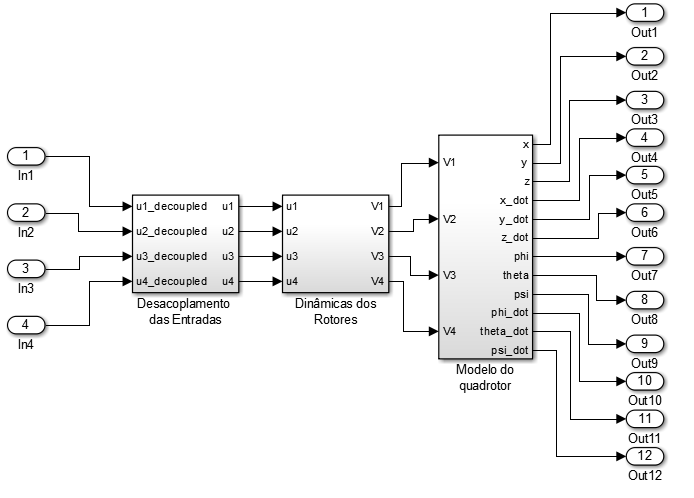
\includegraphics[width=.9\textwidth]{./04-figuras/simulink_drone/diagrama_geral}
%    \label{fig:simulink-drone-diagrama-geral}
%\end{figure}
%
%\begin{figure}[!htb]
%    \centering
%    \caption{Diagrama de blocos representando a simulação do quadrotor para  verificação efeito de sinal em degrau sobre a entrada $u_1$ nos estados afetados por ela}
%    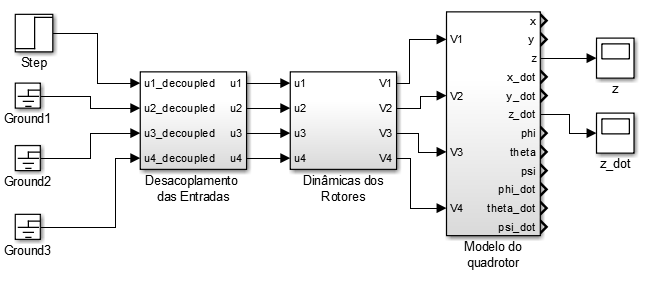
\includegraphics[width=.9\textwidth]{./04-figuras/simulink_drone/diagrama_step_u1}
%    \label{fig:simulink-drone-diagrama-step-u1}
%\end{figure}
%
%\begin{figure}[!htb]
%    \centering
%    \caption{Diagrama de blocos representando a simulação do quadrotor para  verificação efeito de sinal em degrau sobre a entrada $u_2$ nos estados afetados por ela}
%    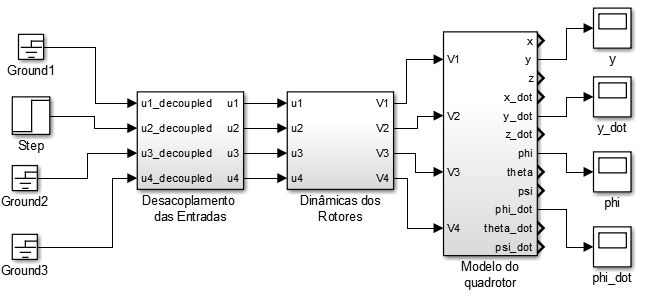
\includegraphics[width=.9\textwidth]{./04-figuras/simulink_drone/diagrama_step_u2}
%    \label{fig:simulink-drone-diagrama-step-u2}
%\end{figure}
%
%\begin{figure}[!htb]
%    \centering
%    \caption{Diagrama de blocos representando a simulação do quadrotor para  verificação efeito de sinal em degrau sobre a entrada $u_3$ nos estados afetados por ela}
%    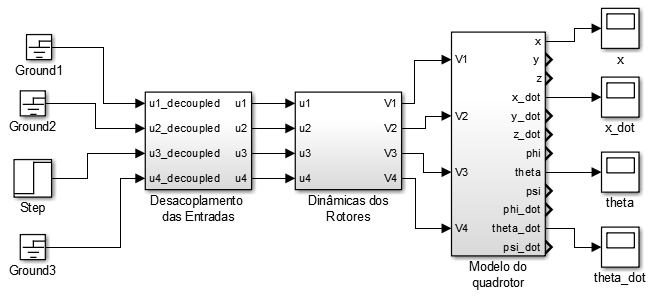
\includegraphics[width=.9\textwidth]{./04-figuras/simulink_drone/diagrama_step_u3}
%    \label{fig:simulink-drone-diagrama-step-u3}
%\end{figure}
%
%\begin{figure}[!htb]
%    \centering
%    \caption{Diagrama de blocos representando a simulação do quadrotor para  verificação efeito de sinal em degrau sobre a entrada $u_4$ nos estados afetados por ela}
%    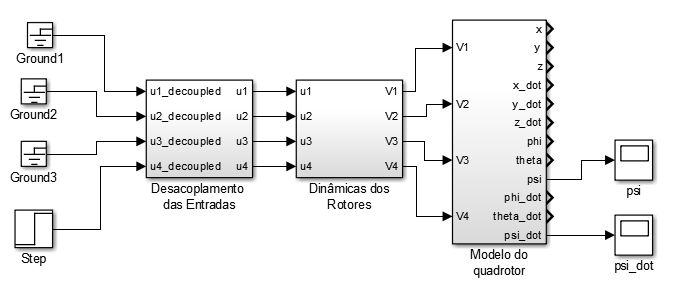
\includegraphics[width=.9\textwidth]{./04-figuras/simulink_drone/diagrama_step_u4}
%    \label{fig:simulink-drone-diagrama-step-u4}
%\end{figure}
%
%%$x$, $\dot{x}$, $\theta$ e $\dot{\theta}$
%
%Num segundo momento, é mostrada a resposta oferecida a uma entrada em degrau pelo quadrotor quando controlado por um controlador PID modelado também por \citeonline{Balas2007}. Neste momento, espera-se que o sistema não divirja e alcance a estabilidade em regime permanente. O mesmo teste é feito mas usando um controlador LQR no lugar do controlador PID. Assim como o controlador PID, o LQR também foi modelado em \citeonline{Balas2007}.
%
%Os ajustes utilizados com os ganhos utilizados na realimentação dos controladores PID e LQR são expostos nas Tabelas \ref{tab:quadrotor-controle-pid} e \ref{tab:quadrotor-controle-lqr}, respectivamente.
%
%\begin{table}[!htb]
    \centering
    \caption{Valores dos ganhos de realimentação do controlador PID projetado para o controle do quadrotor\label{tab:quadrotor-controle-pid}}
    \begin{tabular}{ccccc}
        \cline{2-5}
        & \multicolumn{4}{c}{\textbf{Variáveis controladas}} \\
        
        \hline
        \multicolumn{1}{ c }{\textbf{Variável Realimentada}} & 
                            \textbf{$x$} &
                            \textbf{$y$} & 
                            \textbf{$z$}  & 
                            \textbf{$\psi$} \\
        \hline
        \multicolumn{1}{ c }{\textbf{$\dot{\theta}$}} & 
                            5 &
                            - & 
                            - & 
                            - \\
        \hline
        \multicolumn{1}{ c }{\textbf{$\theta$}} & 
                            37,3 &
                            - & 
                            - & 
                            - \\

        \hline
        \multicolumn{1}{ c }{\textbf{$x$}} & 
                            -10,92 &
                            - & 
                            - & 
                            - \\
        \hline
        \multicolumn{1}{ c }{\textbf{$\dot{x}$}} & 
                            -10,9 &
                            - & 
                            - & 
                            - \\
        \hline
        \multicolumn{1}{ c }{\textbf{$\dot{\phi}$}} & 
                            -  &
                            5 & 
                            - & 
                            - \\
        \hline
        \multicolumn{1}{ c }{\textbf{$\phi$}} & 
                            -  &
                            37,3 & 
                            - & 
                            - \\
        \hline
        \multicolumn{1}{ c }{\textbf{$y$}} & 
                            -  &
                            10,92 & 
                            - & 
                            - \\
        \hline
        \multicolumn{1}{ c }{\textbf{$\dot{y}$}} & 
                            -  &
                            10,9 & 
                            - & 
                            - \\
        \hline
        \multicolumn{1}{ c }{\textbf{$\dot{\psi}$}} & 
                            -  &
                            - & 
                            -10 & 
                            - \\
        \hline
        \multicolumn{1}{ c }{\textbf{$\psi$}} & 
                            -  &
                            - & 
                            -10,6 & 
                            - \\
        \hline
        \multicolumn{1}{ c }{\textbf{$z$}} & 
                            - &
                            - & 
                            - & 
                            3 \\
        \hline
        \multicolumn{1}{ c }{\textbf{$\dot{z}$}} & 
                            - &
                            - & 
                            - & 
                            7,56 \\
        \hline
    \end{tabular}

    \fonte{Adaptado de \citeonline[p.~64]{Balas2007}}
\end{table}

%
%\begin{table}[!htb]
    \centering
    \caption{Valores dos ganhos de realimentação do controlador LQR projetado para o controle do quadrotor\label{tab:quadrotor-controle-lqr}}
    \begin{tabular}{ccccc}
        \cline{2-5}
        & \multicolumn{4}{c}{\textbf{Variáveis controladas}} \\
        
        \hline
        \multicolumn{1}{ c }{\textbf{Variável Realimentada}} & 
                            \textbf{$x$} &
                            \textbf{$y$} & 
                            \textbf{$z$}  & 
                            \textbf{$\psi$} \\
        \hline
        \multicolumn{1}{ c }{\textbf{$\dot{\theta}$}} & 
                            4,3043 &
                            - & 
                            - & 
                            - \\
        \hline
        \multicolumn{1}{ c }{\textbf{$\theta$}} & 
                            25,2884 &
                            - & 
                            - & 
                            - \\

        \hline
        \multicolumn{1}{ c }{\textbf{$x$}} & 
                            -7,8458 &
                            - & 
                            - & 
                            - \\
        \hline
        \multicolumn{1}{ c }{\textbf{$\dot{x}$}} & 
                            -10 &
                            - & 
                            - & 
                            - \\
        \hline
        \multicolumn{1}{ c }{\textbf{$\dot{\phi}$}} & 
                            -  &
                            4,2976 & 
                            - & 
                            - \\
        \hline
        \multicolumn{1}{ c }{\textbf{$\phi$}} & 
                            -  &
                            25,2673 & 
                            - & 
                            - \\
        \hline
        \multicolumn{1}{ c }{\textbf{$y$}} & 
                            -  &
                            7,8431 & 
                            - & 
                            - \\
        \hline
        \multicolumn{1}{ c }{\textbf{$\dot{y}$}} & 
                            -  &
                            10 & 
                            - & 
                            - \\
        \hline
        \multicolumn{1}{ c }{\textbf{$\dot{\psi}$}} & 
                            -  &
                            - & 
                            -15,7751 & 
                            - \\
        \hline
        \multicolumn{1}{ c }{\textbf{$\psi$}} & 
                            -  &
                            - & 
                            -31,6228 & 
                            - \\
        \hline
        \multicolumn{1}{ c }{\textbf{$z$}} & 
                            - &
                            - & 
                            - & 
                            3,9936 \\
        \hline
        \multicolumn{1}{ c }{\textbf{$\dot{z}$}} & 
                            - &
                            - & 
                            - & 
                            10 \\
        \hline
    \end{tabular}

    \fonte{Adaptado de \citeonline[p.~68]{Balas2007}}
\end{table}

%
%\fi

